\documentclass{article}
\usepackage[utf8]{inputenc}
\usepackage{graphicx}

\title{Skin, Touch and Movement}
\author{MCB C61 with Professor David Presti \\ \\ Benjamin Lee}
% \date{8 March 2018}

\begin{document}

\maketitle

\textbf{Key Concepts:}
\begin{itemize}
    \item Somatosensory Receptors
    \item Dorsal-root ganglion
    \item Wilder Penfield
    \item Somatosensory body map
    \item Primary somatosensory cortex (S1)
    \item Two-point descrimination test
    \item Posterior somatosensory cortex (S2, S3, etc)
    \item Neglect Syndrome
    \item Phantom Limb
    \item Primary Motor Cortex (M1)
    \item Supplemnetary motor / premotor areas
    \item Apraxia
    \item Mirror Neurons
    \item Cerebellum
    \item Anosognosia
\end{itemize}

\newpage
\section{The Skin}
The skin is the largest sensory organ. \\
Dendrites of \textbf{somatosensory neurons} (Greek \textit{soma} = body) terminate in the top layers of skin, and the membranes of these nerve fibers contain receptor proteins that respond to touches, pokes, or changes of temperature. \\ 

\begin{figure}[htp]
\centering
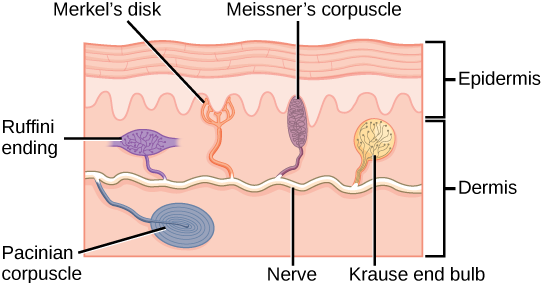
\includegraphics[width=8cm]{images/skin.png}
\caption{Cross section of skin}
\label{fig: skin}
\end{figure}

\noindent Nerve fibers may have \textbf{free endings} on top layer of skin, some are closely associated with hair follicles, and some are structures \textbf{(Merkel's disks, Pacinian corpuscles, Meissner's corpuscles, Ruffini endings)} that respond to the pressure associated with touch. \\

\subsection{Somatosensory Receptors}
\textbf{Touch} response receptors presumed to have \textbf{mechanically-gated ion channels}. (similar to those in the inner ear cells that open as hair bends. \\

\noindent \textbf{Temperature} response receptors are \textbf{TRP receptors} (described in Ch 13, related to perceptions of spicy hot and minty cool) \\
 
\noindent \textbf{Dorsal Root Ganglia (DRG):} clusters of cells near the spinal cord that hold the cell bodies for these nerve fibers. 
\begin{itemize}
    \item DRG nerve fibers in the skin share the same border/adjacent with axons that send signals int he CNS. 
    \item Peripheral dendrites contain voltage-gated sodium and potassium channels and are myelinated. 
    \item When action potenial generated it propagates toward the DRG, bypass the cell body and to the CNS
    \item DRG dendrite functions just like an axon except action potentials propagate toward the cell body. 
\end{itemize}
    
\subsection{Somatosensory Circuitry}
\begin{itemize}
    \item Somatosensory neurons have \textbf{spatial receptive fields}: region of skin where a physical stimulus elicits activity in the specified neuron. 
    \item Axons of DRG synapse with cells in the \textbf{spinal cord} and \textbf{medulla} of the brainstem 
    \item Somatosensory circuitry continues into \textbf{thalamus}
    \item Neurons in thalamus project to \textbf{anterior parietal lobes} in cerebral cortex
    \item Spatial receptive field information is maintained along this pathway to produce a \textbf{somatosensory map} of the body in the parietal lobe. 
    \item Various locations in the body are represented along \textbf{postcentral gyrus}, immediately \textbf{posterior to the central sulcus}. 
\end{itemize}

\subsection{Primary Somatosensory Cortex (S1)}

Like other sensory areas of cortex, the somatosensory cortex receives signals\textbf{ contralaterally} (Signals from left side go to the right brain and vice versa). \\

Lesions in S1 produce loss of sensation in a particular region of the body. Analagous to the visual scotoma (lesion in V1 results in loss of vision to a certain area). \\

\noindent \textbf{Wilder Penfield (1891-1976)} discovered the somatosensory body map while doing brain surgery in the 30s. \\
Electrically stimulated regions of the cerebral cortex while doing brain surgery on patients who were awake. They described the feelings and experiences that they felt. \\

The cortical map is almost exactly how the actual body is mapped: fingers to hand, hand to arm, arm to torso, etc. However, some body parts are completely off from the place they should be, such as the sensory information for \textit{genitals}, which is closer to the foot sensory map and the \textit{face}, which is separate from the neck sensory map and the tongue separate from the face. \\

Somatosensory information density differs between body parts. Fingers and lips have a more densely packed neurons sent to those areas with smaller receptive fields, for keener sense. Other places, such as arms, legs, have poorer somatosensory acuity. \\
Result of densely packed somatosensory dendrites connected to many separate neurons each having small receptive fields and projecting eventually to a region of the parietal lobe (S1) where large numbers of neurons receive the signals. \\

\begin{figure}[htp]
\centering
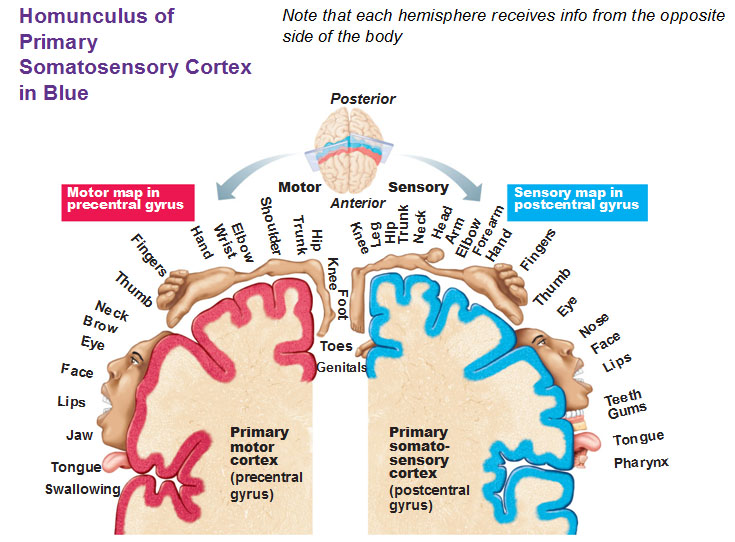
\includegraphics[width=10cm]{images/homunculus.jpg}
\caption{Homunculus: showing more sensory density with larger body parts}
\label{fig: Homunculus}
\end{figure}

\noindent \textbf{Two Point Discrimination Test:} used to measure somatosensory acuity. 
\begin{itemize}
    \item Best done with two people
    \item Take a wire paperclip and bend into a U-shape
    \item Close your eyes and touch the two points on your fingers or lips at the same time
    \item No matter how close the two points are, you can experience two separate points touching your lips or fingertips. (even at 1-2 millimeters apart)
    \item Represents high degree of somatosensory acuity.
    \item When touched on the back, however, the points must be moved at least 1-2 centimeters apart (10 times) before the subject experiences two points. 
    \item Represents low degree of somatosensory acuity. 
\end{itemize}

\subsection{Posterior Somatosensory Cortex (S2, S3, etc)}
Information from the primary somatosensory cortex is sent to other regions of the\textbf{ posterior somatosensory cortex} named S2, S3, etc (analagous to the occipital lobe sending info from V1 to V2, etc). \\

\noindent \textbf{Secondary Somatosensory Cortex:} the collective region of S2, S3, S4, etc. \\

\noindent \textbf{Mice Studies:} Much was learned about the somatosensory cortex by mice. Focusing on the whiskers of the mice\\
Mice depend heavily on their whiskers to collect information, they even have a whisker map in the somatosensory cortex. \\ 

When a \textbf{whisker was cut off}, the sensory information from that whisker is no longer sent to the part of the sensory map that it responded with. However, that section of the brain doesn't die or stay idle; it instead \textbf{connects with adjacent whiskers}, making them more sensitive. This involves the \underline{growing and branching of axons and dendrites} to strengthen connections! (\textbf{Neuroplasiticity!!}) \\

\noindent \textbf{Phantom Limb:} similar to the amputated whisker, amputated limbs of humans produces the same effect. So if an arm was amputated, the neurons in that section would connect with the face and shoulder neurons in that region. Likely cause of \textit{phantom limb} because the neurons that activate in that area would activate the same arm neurons that used to be there. 

V.S. Ramachandran, a neuroscientist at UC San Diego, experimented with phantom limbs. \\
Touched the face of patients and they felt him touch their phantom limb. Dropping water on their face resulted in them feeling water drop down their arm. \\

\section{Primary Motor Cortex (M1)} 
Body map of neurons that send out signals that initiate the contraction of skeletal muscles, involved in the movements of our body. \\

Neurons in M1 fire and the signals propagate via the spinal cord getting to the synapses with muscles of the body and neuromuscular junction (NMJ). \textbf{Acetylcholine} is released at these junctions, making muscle fibers contract. \\

\noindent \textbf{Contralateral} connection between M1 and the body
\begin{itemize}
    \item Right posterior frontal lobe's (M1) controls movement of the left side of the body
    \item Left Posterior frontal lobe's (M1) controls movement of the right side of the body
    \item Lesions in M1 produce inability to move muscles associated with corresponding part (possibly \textbf{paralysis}) 
\end{itemize}

\subsection{Supplementary Motor Areas (Premotor Areas)}
Anterior to M1 in the frontal lobes involved with control of body movement. \\
This area is involved in planning and sequencing muscles movements, neurons here fire before M1 signals. \\

\noindent Lesions in this area don't result in paralysis but \textbf{disorganized movemen}t. \\
\textbf{Apraxias:} disorders in the organization of movements. \\

\noindent Sensory-motor interconnectivity neurons are in the premotor and frontal lobes \\

\noindent \textbf{Mirror Neurons:} Visual perception of an action fires the same neurons that perform the action. (eating a banana, monkey see monkey do) \\

\subsection{Cerebellum}
Centrally involved in the regulation of movement. wrapped around the brainstem and is very densely packed with neurons and neural connections. About 50 billion neurons. More neurons in cerebellum than in the rest of brain. \\

\textbf{Purkinje cell} type of cerebellar neuron. Each cell has several hundred thousand dendritic spines receiving input from other neurons. \\

Cerebellum involved in the \textbf{timing} and \textbf{coordination} of movement. Individuals who have sustained damage to crerebellum are not paralyzed, but they are impaired in tehir ability to smoothly execute movements. Jerky, clumsy movement. \\

\noindent \textbf{Neglect Syndrome:} when damage to one side of the hemisphere (or both), there is a deficit in attention to the contralateral side of that field of vision. \\

\noindent \textbf{Anosognosia:} Lack of knowledge of ones own disease. \\ 
Common in people who have strokes or lesions due to strokes. \\


















\end{document}